% A three-state Markov chain with its transition probabilities. Generated by a short script.
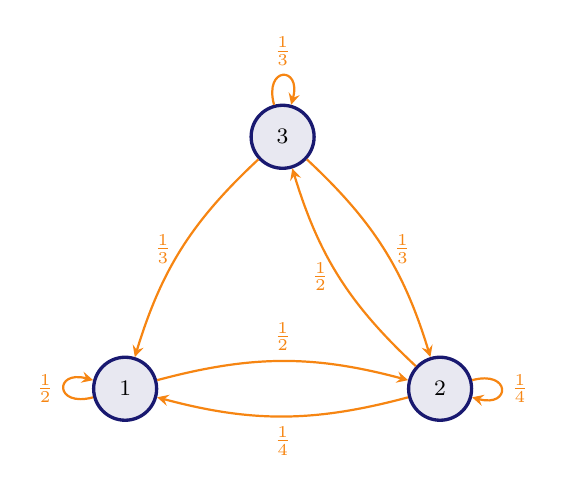
\begin{tikzpicture}[>=stealth,every node/.style={font=\footnotesize},st/.style={circle,draw=MidnightBlue,very thick,fill=MidnightBlue!10,minimum size=8mm}]
\node[st] (a) at (0,0) {$1$};
\node[st] (b) at (4,0) {$2$};
\node[st] (c) at (2,3.2) {$3$};
\draw[->,thick,BurntOrange] (a) to[bend left=15] node[above] {$\frac12$} (b);
\draw[->,thick,BurntOrange] (b) to[bend left=15] node[below] {$\frac14$} (a);
\draw[->,thick,BurntOrange] (b) to[bend left=15] node[left] {$\frac12$} (c);
\draw[->,thick,BurntOrange] (c) to[bend left=15] node[right] {$\frac13$} (b);
\draw[->,thick,BurntOrange] (c) to[bend right=15] node[left] {$\frac13$} (a);
\draw[->,thick,BurntOrange] (a) to[loop left,looseness=6] node[left] {$\frac12$} (a);
\draw[->,thick,BurntOrange] (b) to[loop right,looseness=6] node[right] {$\frac14$} (b);
\draw[->,thick,BurntOrange] (c) to[loop above,looseness=6] node[above] {$\frac13$} (c);
\end{tikzpicture}
